\documentclass[11pt]{article}

\usepackage{graphicx}
\usepackage{hyperref}
\usepackage{natbib}
\usepackage{amsmath}

\bibliographystyle{plain}  % or unsrt, alpha, etc.
\setlength{\textwidth}{6.5in}
\setlength{\headheight}{0in}
\setlength{\textheight}{8.0in}
\setlength{\hoffset}{0in}
\setlength{\voffset}{0in}
\setlength{\oddsidemargin}{0in}
\setlength{\evensidemargin}{0in}


\title{Computational Physics -  Problem Set 3}
  
\author{Frederik Holst Knudsen}


\begin{document}

\maketitle
Github URL: https://github.com/frederikholst/phys-ga2000
\section{Matrix Multiplication}
The matrix product of two NxN matrices is computed using nested for loops and np.dot method respectively. See Figure \ref*{MM}.

\begin{figure}[!htbp]
    \centering
    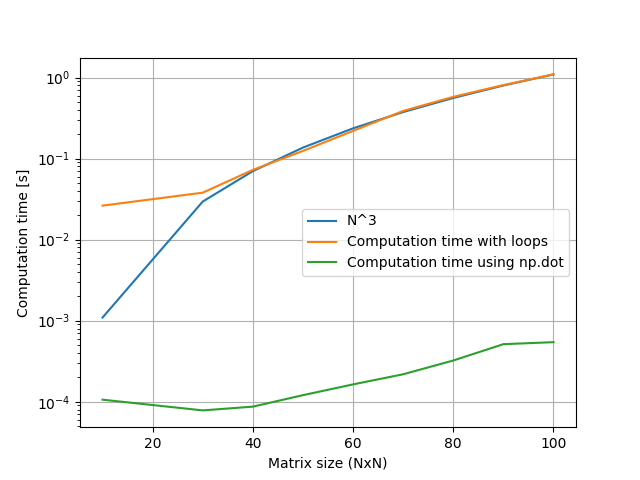
\includegraphics[width=0.7\textwidth]{loops_comp.png}
    \caption{The computation time is plotted in log scale against the matrix size N, so that the matrices has sizes NxN. The matrix elements are random numbers. The $N^3$ graph is normalized against the nested for-loop computation and shows very good agreement. One notices how the np.dot method is much faster than the nested loop method.}
    \label{MM}
\end{figure}


\section{Decay}
The decay of Bi-213 to Bi-209 has been simulated and the populations over a time interval of 20,000 seconds are shown in figure \ref{dec}.
\begin{figure}[!htbp]
    \centering
    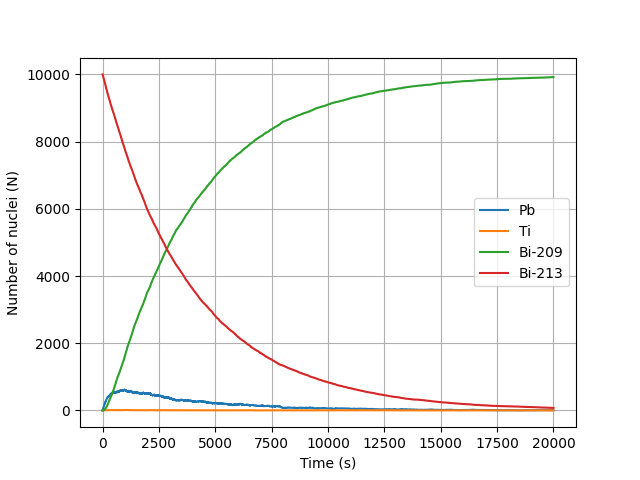
\includegraphics[width=0.7\textwidth]{Decay.png}
    \caption{Simulation of the population of the four different populations, Ti, Bi-213, Bi-209 and Pb, for a series of decays where Bi-213 can decay to Bi-209 either via Ti-Pb-Bi or directly via Pb-Bi.}
    \label{dec}
\end{figure}

\section{Decay 2: Non-uniform distribution}
We use a non-uniform distribution,

$$ P(t)dt=2^{-t/\tau}\frac{\ln{2}}{\tau}dt $$

to calculate the decay of a sample of N atoms, as a different and more effective method than the one shown above. We use a uniform distribution of random numbers from 0 to 1, z and map those onto the non-uniform distribution x. Using the transformation method presented in Newman ch. 10, we have the mapping between the two distributions x and z to be:

$$ x=-\frac{1}{\mu}\ln{(1-z)} $$

After sorting the values, we ask for each time interval (from 0 to 2000 seconds) how many atoms haven't decayed yet. This defines the decay graph shown in figure \ref{dec2}.
\begin{figure}[!htbp]
    \centering
    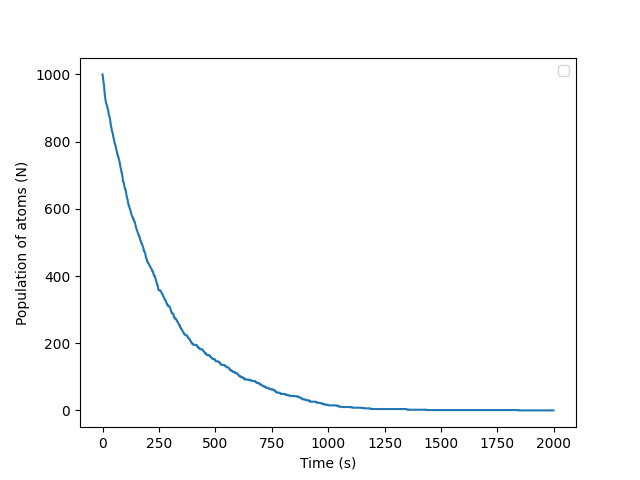
\includegraphics[width=0.7\textwidth]{decay2.png}
    \caption{Simulation of the population decay of Ti-208 made using the transformation method of generating 1000 random numbers from a nonuniform distribution. The graph shows how many atoms have not decayed yet at a given point in time.}
    \label{dec2}
\end{figure}


\section{The Central Limit Theorem}
First we carry out the derivations:
The theoretical mean of y is found by noting that the mean of the $x_i$ is equal to one:
\begin{align}
    E[y] &= N^{-1}\sum_{i=1}^{N}E[x_i] \\
    &= N^{-1}N = 1
\end{align}

For finding the variance, we use that $Var[x_i]=1$ and that the variance of a constant gives the square of that constant:

\begin{align}
    Var[y]&=\frac{1}{N^2}\sum_{i=1}^{N}Var[x_i]\\
    &=\frac{1}{N^2}N=N
\end{align}


Then we use a sample size of 1000 for each of the N values. For every N, we compute the distribution of y and see that in the limit of large N, the distribution becomes a Gaussian, see Figure \ref*{gaus}. For a plot of how the mean, skewness, variance and kurtosis varies with N, see figure \ref*{feat}. 


The skewness becomes less than 1 percent of the case for $N=1$ at $N=211$ and likewise for the kurtosis at $N=41$.

\begin{figure}[!htbp]
    \centering
    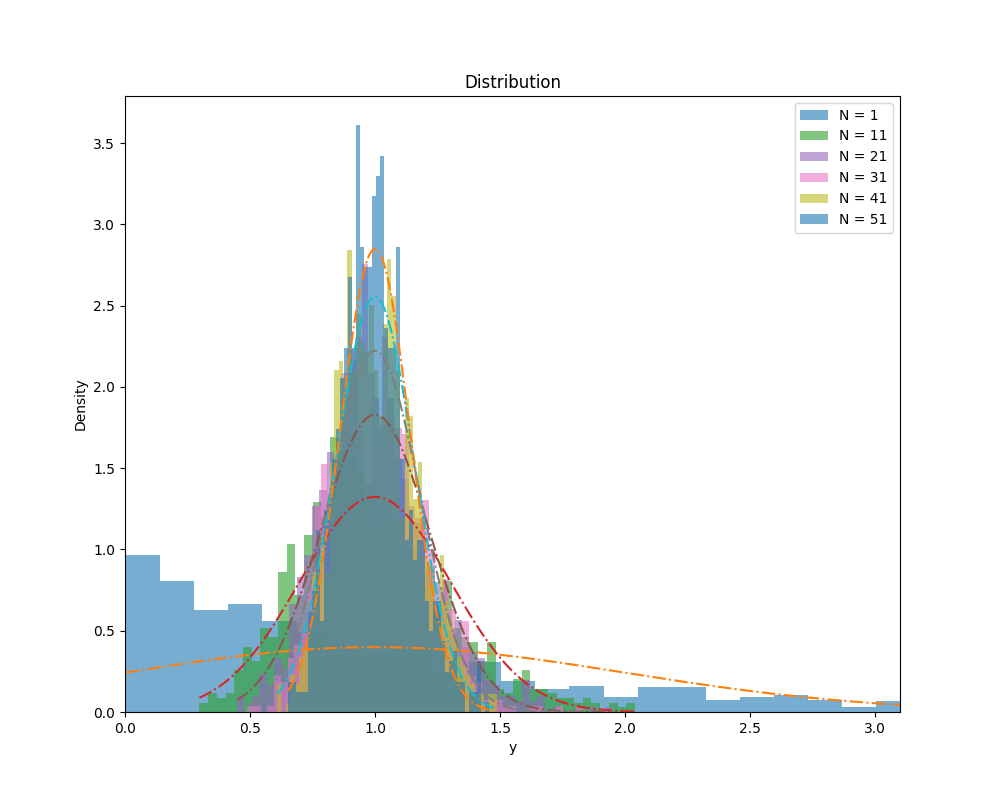
\includegraphics[width=0.7\textwidth]{gaus.png}
    \caption{For larger and larger N, a histogram (bin number = 50), is plotted. For every distribution, the mean is 1. For large N, the distribution is in good agreement with the Gaussian (dashed line).}
    \label{gaus}
\end{figure}


\begin{figure}[!htbp]
    \centering
    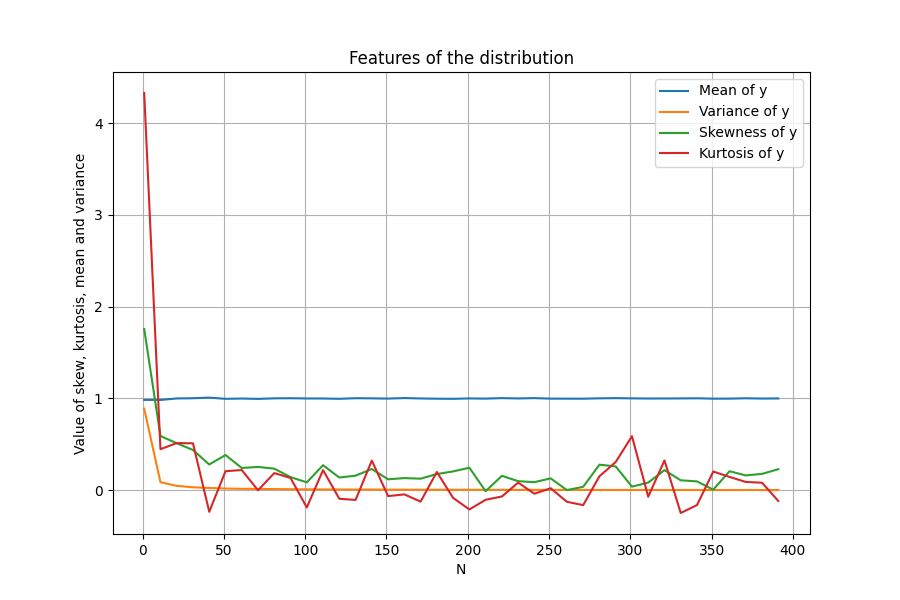
\includegraphics[width=0.7\textwidth]{distribution_feat.png}
    \caption{Each graph shows the N-depedence of mean, variance, kurtosis and skewness respectively. We see that mean=1 as expected, and that the other three vanishes for large N.}
    \label{feat}
\end{figure}



\end{document}



